\chapter{Uruchomienie gry}
\thispagestyle{chapterBeginStyle}

Kod źródłowy programu, wraz z plikami wykonywalnymi gry, znajduje się na załączonej płycie CD, oraz online w repozytorium GitHub \cite{Github}.

\section{Struktura plików}
Struktura plików wygląda następująco:\\
\begin{algorithm}[H]
    $./$\\
    $|\textit{| Kod\_Źródłowy/}$\\
    $|\hskip2em |\textit{| Assets/}$\\
    $|$\\
    $|\textit{| Gra/}$\\
    $|\hskip2em |\textit{| Windows/}$\\
    $|\hskip2em |\textit{| Linux/}$\\
    $|$\\
    $|\textit{| Praca\_Inżynierska.pdf}$\\
\end{algorithm}

\section{Uruchomienie gry}
    Wewnątrz folderu $Gra$ znajdują się pliki wykonywalne, pozwalające na uruchomienie gry.\\
    \textbf{Windows}\\
    Gra została przetestowana na systemie Windows 10. Aby uruchomić grę należy uruchomić plik\\
    $Gra/Windows/gra.exe$.\\
    \textbf{Linux}\\
    Gra została przetestowana na systemie Ubuntu 20.04. Aby uruchomić grę należy uruchomić plik\\
    $Gra/Linux/gra.x86\_64$.\\

\section{Kod źródłowy}
    Program został stworzony z wykorzystaniem silnika Unity, który sam dodaje znaczną ilość kodu, 
    dlatego w katalogu $\textit{Kod\_Źródłowy}$ został załączony jedynie folder zawierający autorską część kodu. \\
    Wewnątrz znajduje się również folder $\textit{Assets/Other\_Assets}$ zawierający zaimportowane modele 3D 
    ze sklepu Unity \cite{UnityAssetStore}.\\
    \vspace{2cm}\\
    Aby uruchomić grę z kodu źródłowego, należy:
    \begin{itemize}
        \item zainstalować program UnityHub zgodnie z instrukcjami z oficjalnej strony \cite{UnityInstallation}.
        \item zainstalować pakiet Ml-Agents \cite{UnityMlAgentsInstallation}.
        \item uruchomić Unity i stworzyć nowy projekt.
        \item podmienić folder $Assets$ w nowym projekcie na pobrany folder $\textit{Kod\_Źródłowy/Assets/}$.
        \item załadować scenę $Scenes/MainMenu$, oraz uruchomić.
    \end{itemize}

\section{Poruszanie się w grze}
    Po uruchomieniu gry użytkownikowi prezentowany jest ekran główny, wraz z dwiema opcjami. Pierwsza z nich pozwala na rozpoczęcie gry, 
    natomiast druga - na utworzenie własnego terenu do gry.
    \begin{figure}[H]
        \centering
        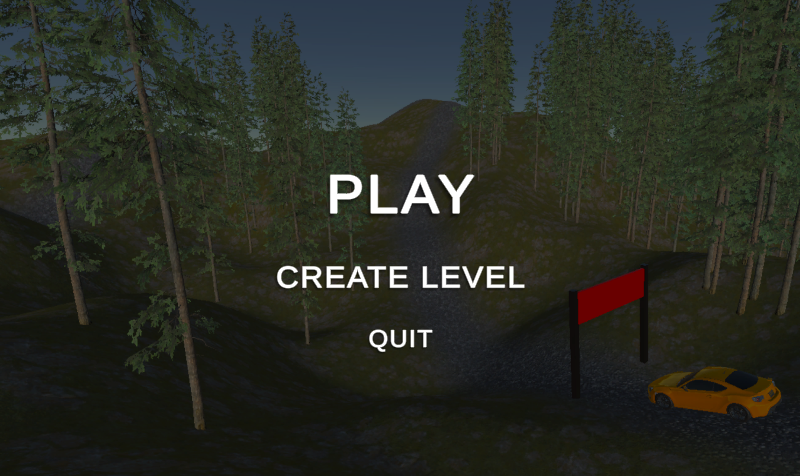
\includegraphics[width=.7\textwidth]{figures/game_instruction_start.png}
        \caption{Instruckja grania - ekran główny}
        \label{fig}
    \end{figure}
    Jeżeli użytkownik wybierze opcję gry, na kolejnym etapie zostanie poproszony o wybór poziomu oraz terenu. 
    Tereny utworzone przez użytkownika też pojawią się poniższym menu rozwijanym.
    \begin{figure}[H]
        \centering
        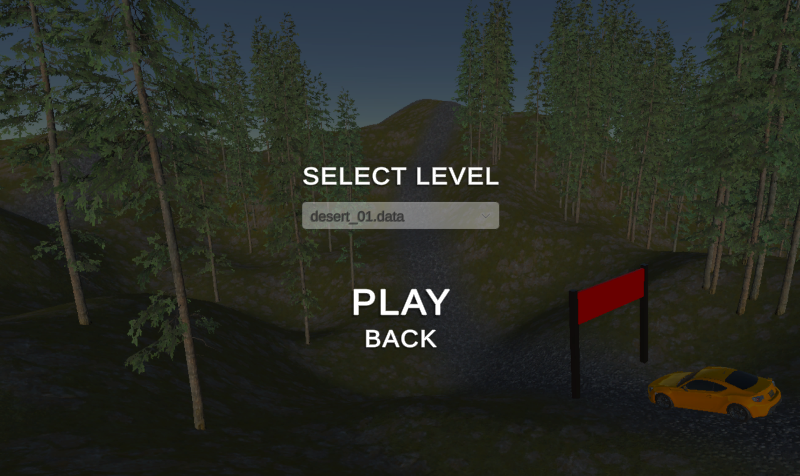
\includegraphics[width=.7\textwidth]{figures/game_instruction_choose_level.png}
        \caption{Instruckja grania - ekran główny}
        \label{fig}
    \end{figure}
    \clearpage
    Po włączeniu gry, wyścig rozpoczyna się od razu po dotknięciu ziemi. Do kontroli pojazdu należy używać strzałek na klawiaturze.
    \begin{figure}[H]
        \centering
        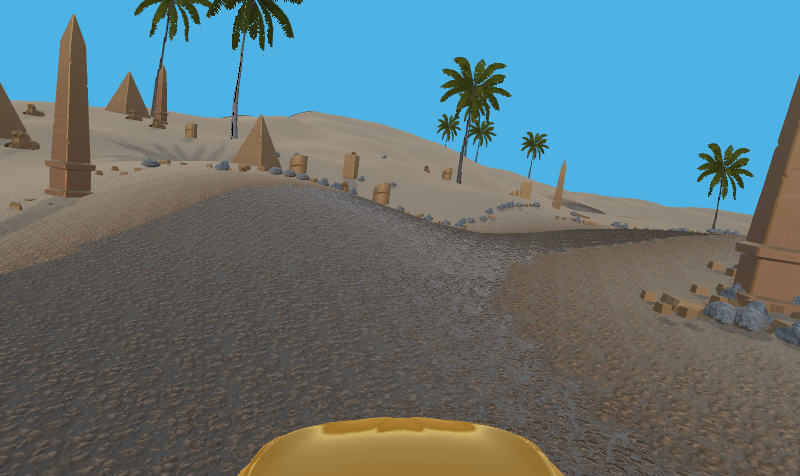
\includegraphics[width=.7\textwidth]{figures/game_instruction_play.png}
        \caption{Instruckja grania - ekran główny}
        \label{fig}
    \end{figure}
    Aby zatrzymać wyścig w trakcie, należy wcisnąć przycisk $Escape$ na klawiaturze. Czas w grze zostanie zatrzymany aż do wyłączenia widocznego menu.
    Można to osiągnąć wciskając ponownie $Escape$, lub wybierając opcję $Resume$ w menu. Dodatkowo użytkownik ma możliwość zakończyć grę i powrócić
    do głównego menu.
    \begin{figure}[H]
        \centering
        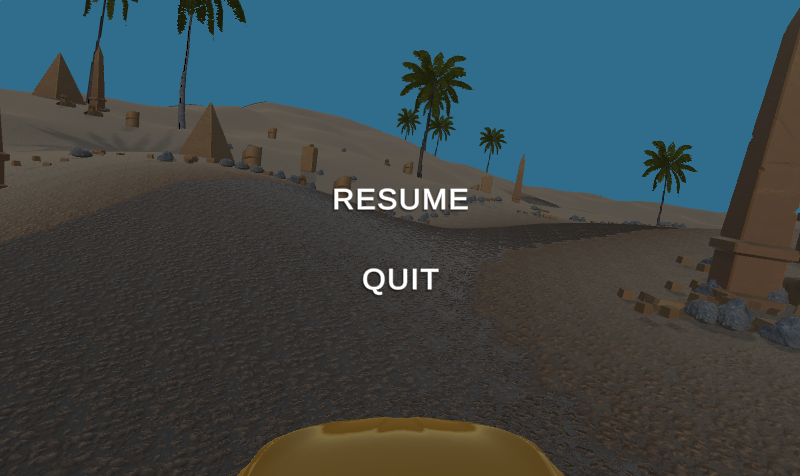
\includegraphics[width=.7\textwidth]{figures/game_instruction_pause.png}
        \caption{Instruckja grania - ekran główny}
        \label{fig}
    \end{figure}
    \clearpage
    Oprócz domyślnie zdefiniowanych poziomów i terenów, użytkownik ma możliwość wygenerować własną trasę, za pomocą kilku parametrów:
    \begin{itemize}
        \item Parametry $Complexity$ i $Seed$ definiują jak bardzo kręta będzie droga.
        \item Parametry $Details$, $Scale$ i $Offset$ pozwalają na określenie kształtu terenu.
        \item Parametr $Terrain$ określa szatę graficzną terenu.
    \end{itemize}
    Aby podejrzeć trasę z różnych stron można wykorzystać suwak $Preview Rotation$.\\
    Po ustawieniu wybranych parametrów, należy ustawić nazwę pliku w polu $Filename$. Pod taką nazwą pojawi się 
    wygenerowany teren podczas wyboru poziomu przed grą. Następnie należy kliknąć przycisk $Save$ aby zapisać teren.
    \begin{figure}[H]
        \centering
        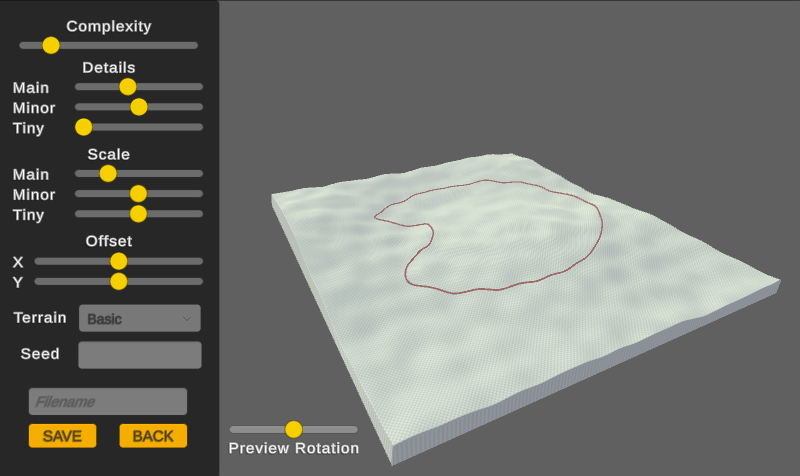
\includegraphics[width=.7\textwidth]{figures/game_instruction_create.png}
        \caption{Instruckja grania - ekran główny}
        \label{fig}
    \end{figure}